\section{TiXmlString Class Reference}
\label{classTiXmlString}\index{TiXmlString@{TiXmlString}}
{\tt \#include $<$tinystr.h$>$}

Inheritance diagram for TiXmlString::\begin{figure}[H]
\begin{center}
\leavevmode
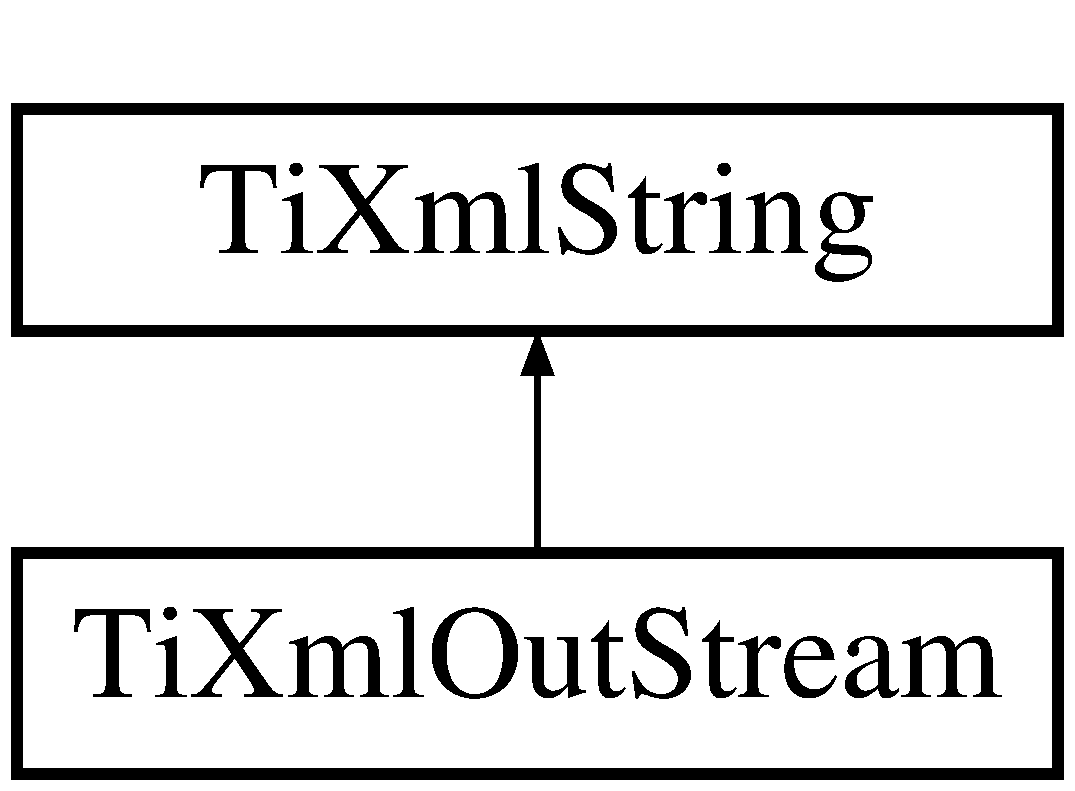
\includegraphics[height=2cm]{classTiXmlString}
\end{center}
\end{figure}
\subsection*{Public Types}
\begin{CompactItemize}
\item 
typedef size\_\-t {\bf size\_\-type}
\end{CompactItemize}
\subsection*{Public Member Functions}
\begin{CompactItemize}
\item 
{\bf TiXmlString} ()
\item 
{\bf TiXmlString} (const {\bf TiXmlString} \&copy)
\item 
TIXML\_\-EXPLICIT {\bf TiXmlString} (const char $\ast$copy)
\item 
TIXML\_\-EXPLICIT {\bf TiXmlString} (const char $\ast$str, {\bf size\_\-type} len)
\item 
{\bf $\sim$TiXmlString} ()
\item 
{\bf TiXmlString} \& {\bf operator=} (const char $\ast$copy)
\item 
{\bf TiXmlString} \& {\bf operator=} (const {\bf TiXmlString} \&copy)
\item 
{\bf TiXmlString} \& {\bf operator+=} (const char $\ast$suffix)
\item 
{\bf TiXmlString} \& {\bf operator+=} (char single)
\item 
{\bf TiXmlString} \& {\bf operator+=} (const {\bf TiXmlString} \&suffix)
\item 
const char $\ast$ {\bf c\_\-str} () const 
\item 
const char $\ast$ {\bf data} () const 
\item 
{\bf size\_\-type} {\bf length} () const 
\item 
{\bf size\_\-type} {\bf size} () const 
\item 
bool {\bf empty} () const 
\item 
{\bf size\_\-type} {\bf capacity} () const 
\item 
const char \& {\bf at} ({\bf size\_\-type} index) const 
\item 
char \& {\bf operator[$\,$]} ({\bf size\_\-type} index) const 
\item 
{\bf size\_\-type} {\bf find} (char lookup) const 
\item 
{\bf size\_\-type} {\bf find} (char tofind, {\bf size\_\-type} offset) const 
\item 
void {\bf clear} ()
\item 
void {\bf reserve} ({\bf size\_\-type} cap)
\item 
{\bf TiXmlString} \& {\bf assign} (const char $\ast$str, {\bf size\_\-type} len)
\item 
{\bf TiXmlString} \& {\bf append} (const char $\ast$str, {\bf size\_\-type} len)
\item 
void {\bf swap} ({\bf TiXmlString} \&other)
\end{CompactItemize}
\subsection*{Static Public Attributes}
\begin{CompactItemize}
\item 
static const {\bf size\_\-type} {\bf npos} = static\_\-cast$<$ {\bf TiXmlString::size\_\-type} $>$(-1)
\end{CompactItemize}
\subsection*{Classes}
\begin{CompactItemize}
\item 
struct \textbf{Rep}
\end{CompactItemize}


\subsection{Member Typedef Documentation}
\index{TiXmlString@{TiXmlString}!size\_\-type@{size\_\-type}}
\index{size\_\-type@{size\_\-type}!TiXmlString@{TiXmlString}}
\subsubsection{\setlength{\rightskip}{0pt plus 5cm}typedef size\_\-t {\bf TiXmlString::size\_\-type}}\label{classTiXmlString_beb2c1893a04c17904f7c06546d0b971}




\subsection{Constructor \& Destructor Documentation}
\index{TiXmlString@{TiXmlString}!TiXmlString@{TiXmlString}}
\index{TiXmlString@{TiXmlString}!TiXmlString@{TiXmlString}}
\subsubsection{\setlength{\rightskip}{0pt plus 5cm}TiXmlString::TiXmlString ()\hspace{0.3cm}{\tt  [inline]}}\label{classTiXmlString_342f61e0fc2244df300b73aedf6d3fef}


\index{TiXmlString@{TiXmlString}!TiXmlString@{TiXmlString}}
\index{TiXmlString@{TiXmlString}!TiXmlString@{TiXmlString}}
\subsubsection{\setlength{\rightskip}{0pt plus 5cm}TiXmlString::TiXmlString (const {\bf TiXmlString} \& {\em copy})\hspace{0.3cm}{\tt  [inline]}}\label{classTiXmlString_c80fe17693a438c9ab2591664743fcb6}


\index{TiXmlString@{TiXmlString}!TiXmlString@{TiXmlString}}
\index{TiXmlString@{TiXmlString}!TiXmlString@{TiXmlString}}
\subsubsection{\setlength{\rightskip}{0pt plus 5cm}TIXML\_\-EXPLICIT TiXmlString::TiXmlString (const char $\ast$ {\em copy})\hspace{0.3cm}{\tt  [inline]}}\label{classTiXmlString_a3b32bd2891a757c9f36c21db44c81d2}


\index{TiXmlString@{TiXmlString}!TiXmlString@{TiXmlString}}
\index{TiXmlString@{TiXmlString}!TiXmlString@{TiXmlString}}
\subsubsection{\setlength{\rightskip}{0pt plus 5cm}TIXML\_\-EXPLICIT TiXmlString::TiXmlString (const char $\ast$ {\em str}, {\bf size\_\-type} {\em len})\hspace{0.3cm}{\tt  [inline]}}\label{classTiXmlString_4b17ea5c5db986f14827223dfa8f1547}


\index{TiXmlString@{TiXmlString}!$\sim$TiXmlString@{$\sim$TiXmlString}}
\index{$\sim$TiXmlString@{$\sim$TiXmlString}!TiXmlString@{TiXmlString}}
\subsubsection{\setlength{\rightskip}{0pt plus 5cm}TiXmlString::$\sim$TiXmlString ()\hspace{0.3cm}{\tt  [inline]}}\label{classTiXmlString_7ac03f581ca3422c4808162ab14f3450}




\subsection{Member Function Documentation}
\index{TiXmlString@{TiXmlString}!operator=@{operator=}}
\index{operator=@{operator=}!TiXmlString@{TiXmlString}}
\subsubsection{\setlength{\rightskip}{0pt plus 5cm}{\bf TiXmlString}\& TiXmlString::operator= (const char $\ast$ {\em copy})\hspace{0.3cm}{\tt  [inline]}}\label{classTiXmlString_e0bc6147afc0ec2aa0da3a3c0a8fcfb0}


\index{TiXmlString@{TiXmlString}!operator=@{operator=}}
\index{operator=@{operator=}!TiXmlString@{TiXmlString}}
\subsubsection{\setlength{\rightskip}{0pt plus 5cm}{\bf TiXmlString}\& TiXmlString::operator= (const {\bf TiXmlString} \& {\em copy})\hspace{0.3cm}{\tt  [inline]}}\label{classTiXmlString_b1f1f5d3eceaa0f22d0a7e6055ea81b0}


\index{TiXmlString@{TiXmlString}!operator+=@{operator+=}}
\index{operator+=@{operator+=}!TiXmlString@{TiXmlString}}
\subsubsection{\setlength{\rightskip}{0pt plus 5cm}{\bf TiXmlString}\& TiXmlString::operator+= (const char $\ast$ {\em suffix})\hspace{0.3cm}{\tt  [inline]}}\label{classTiXmlString_b56336ac2aa2a08d24a71eb9a2b502a5}


\index{TiXmlString@{TiXmlString}!operator+=@{operator+=}}
\index{operator+=@{operator+=}!TiXmlString@{TiXmlString}}
\subsubsection{\setlength{\rightskip}{0pt plus 5cm}{\bf TiXmlString}\& TiXmlString::operator+= (char {\em single})\hspace{0.3cm}{\tt  [inline]}}\label{classTiXmlString_6aa09d5240470b76d54ec709e04f8c13}


\index{TiXmlString@{TiXmlString}!operator+=@{operator+=}}
\index{operator+=@{operator+=}!TiXmlString@{TiXmlString}}
\subsubsection{\setlength{\rightskip}{0pt plus 5cm}{\bf TiXmlString}\& TiXmlString::operator+= (const {\bf TiXmlString} \& {\em suffix})\hspace{0.3cm}{\tt  [inline]}}\label{classTiXmlString_fdcae5ea2b4d9e194dc21226b817f417}


\index{TiXmlString@{TiXmlString}!c\_\-str@{c\_\-str}}
\index{c\_\-str@{c\_\-str}!TiXmlString@{TiXmlString}}
\subsubsection{\setlength{\rightskip}{0pt plus 5cm}const char$\ast$ TiXmlString::c\_\-str () const\hspace{0.3cm}{\tt  [inline]}}\label{classTiXmlString_5581ca641d915551d3cda90f8e7bf49b}


\index{TiXmlString@{TiXmlString}!data@{data}}
\index{data@{data}!TiXmlString@{TiXmlString}}
\subsubsection{\setlength{\rightskip}{0pt plus 5cm}const char$\ast$ TiXmlString::data () const\hspace{0.3cm}{\tt  [inline]}}\label{classTiXmlString_00abc60f135c7ca1951c7334cc2c7993}


\index{TiXmlString@{TiXmlString}!length@{length}}
\index{length@{length}!TiXmlString@{TiXmlString}}
\subsubsection{\setlength{\rightskip}{0pt plus 5cm}{\bf size\_\-type} TiXmlString::length () const\hspace{0.3cm}{\tt  [inline]}}\label{classTiXmlString_3202f27d139a3fac79205f1f3c707727}


\index{TiXmlString@{TiXmlString}!size@{size}}
\index{size@{size}!TiXmlString@{TiXmlString}}
\subsubsection{\setlength{\rightskip}{0pt plus 5cm}{\bf size\_\-type} TiXmlString::size () const\hspace{0.3cm}{\tt  [inline]}}\label{classTiXmlString_96103e5c0f67e987fa48527e1f47a1f6}


\index{TiXmlString@{TiXmlString}!empty@{empty}}
\index{empty@{empty}!TiXmlString@{TiXmlString}}
\subsubsection{\setlength{\rightskip}{0pt plus 5cm}bool TiXmlString::empty () const\hspace{0.3cm}{\tt  [inline]}}\label{classTiXmlString_9a61e1d11cdb71bea4a4ed79caa793f4}


\index{TiXmlString@{TiXmlString}!capacity@{capacity}}
\index{capacity@{capacity}!TiXmlString@{TiXmlString}}
\subsubsection{\setlength{\rightskip}{0pt plus 5cm}{\bf size\_\-type} TiXmlString::capacity () const\hspace{0.3cm}{\tt  [inline]}}\label{classTiXmlString_76e4d6aba7845f4cf9c02332a5fbf916}


\index{TiXmlString@{TiXmlString}!at@{at}}
\index{at@{at}!TiXmlString@{TiXmlString}}
\subsubsection{\setlength{\rightskip}{0pt plus 5cm}const char\& TiXmlString::at ({\bf size\_\-type} {\em index}) const\hspace{0.3cm}{\tt  [inline]}}\label{classTiXmlString_6763093267bbdecbf03f8840bc349877}


\index{TiXmlString@{TiXmlString}!operator[]@{operator[]}}
\index{operator[]@{operator[]}!TiXmlString@{TiXmlString}}
\subsubsection{\setlength{\rightskip}{0pt plus 5cm}char\& TiXmlString::operator[$\,$] ({\bf size\_\-type} {\em index}) const\hspace{0.3cm}{\tt  [inline]}}\label{classTiXmlString_e8cdc1d46c538536b786f7ae03c0c1d9}


\index{TiXmlString@{TiXmlString}!find@{find}}
\index{find@{find}!TiXmlString@{TiXmlString}}
\subsubsection{\setlength{\rightskip}{0pt plus 5cm}{\bf size\_\-type} TiXmlString::find (char {\em lookup}) const\hspace{0.3cm}{\tt  [inline]}}\label{classTiXmlString_5c2b368b5eafe075fd9565cbcbd4c2f9}


\index{TiXmlString@{TiXmlString}!find@{find}}
\index{find@{find}!TiXmlString@{TiXmlString}}
\subsubsection{\setlength{\rightskip}{0pt plus 5cm}{\bf size\_\-type} TiXmlString::find (char {\em tofind}, {\bf size\_\-type} {\em offset}) const\hspace{0.3cm}{\tt  [inline]}}\label{classTiXmlString_5f2a6fd565751410b392f249a9786db4}


\index{TiXmlString@{TiXmlString}!clear@{clear}}
\index{clear@{clear}!TiXmlString@{TiXmlString}}
\subsubsection{\setlength{\rightskip}{0pt plus 5cm}void TiXmlString::clear ()\hspace{0.3cm}{\tt  [inline]}}\label{classTiXmlString_b20e06e4c666abf3bdbfb3a1191d4888}


\index{TiXmlString@{TiXmlString}!reserve@{reserve}}
\index{reserve@{reserve}!TiXmlString@{TiXmlString}}
\subsubsection{\setlength{\rightskip}{0pt plus 5cm}void TiXmlString::reserve ({\bf size\_\-type} {\em cap})}\label{classTiXmlString_88ecf9f0f00cb5c67b6b637958d7049c}


\index{TiXmlString@{TiXmlString}!assign@{assign}}
\index{assign@{assign}!TiXmlString@{TiXmlString}}
\subsubsection{\setlength{\rightskip}{0pt plus 5cm}{\bf TiXmlString} \& TiXmlString::assign (const char $\ast$ {\em str}, {\bf size\_\-type} {\em len})}\label{classTiXmlString_c72f3d9149b7812c1e6c59402014d0d5}


\index{TiXmlString@{TiXmlString}!append@{append}}
\index{append@{append}!TiXmlString@{TiXmlString}}
\subsubsection{\setlength{\rightskip}{0pt plus 5cm}{\bf TiXmlString} \& TiXmlString::append (const char $\ast$ {\em str}, {\bf size\_\-type} {\em len})}\label{classTiXmlString_d44b21700d2ec24a511367b222b643fb}


\index{TiXmlString@{TiXmlString}!swap@{swap}}
\index{swap@{swap}!TiXmlString@{TiXmlString}}
\subsubsection{\setlength{\rightskip}{0pt plus 5cm}void TiXmlString::swap ({\bf TiXmlString} \& {\em other})\hspace{0.3cm}{\tt  [inline]}}\label{classTiXmlString_a392cbc180752a79f007f4f9280c7762}




\subsection{Member Data Documentation}
\index{TiXmlString@{TiXmlString}!npos@{npos}}
\index{npos@{npos}!TiXmlString@{TiXmlString}}
\subsubsection{\setlength{\rightskip}{0pt plus 5cm}const {\bf TiXmlString::size\_\-type} {\bf TiXmlString::npos} = static\_\-cast$<$ {\bf TiXmlString::size\_\-type} $>$(-1)\hspace{0.3cm}{\tt  [static]}}\label{classTiXmlString_8f4422d227088dc7bec96f479b275d0a}




The documentation for this class was generated from the following files:\begin{CompactItemize}
\item 
/home/msneddon/eclipse/ganymede\_\-cpp/workspace/NFsim\_\-svn/src/NFinput/TinyXML/{\bf tinystr.h}\item 
/home/msneddon/eclipse/ganymede\_\-cpp/workspace/NFsim\_\-svn/src/NFinput/TinyXML/{\bf tinystr.cpp}\end{CompactItemize}
